% Этот шаблон документа разработан в 2014 году
% Данилом Фёдоровых (danil@fedorovykh.ru) 
% для использования в курсе 
% <<Документы и презентации в \LaTeX>>, записанном НИУ ВШЭ
% для Coursera.org: http://coursera.org/course/latex .
% Исходная версия шаблона --- 
% https://www.writelatex.com/coursera/latex/3.2

\documentclass[a4paper,12pt]{article}

%%% Работа с русским языком
\usepackage{cmap}					% поиск в PDF
\usepackage{mathtext} 				% русские буквы в формулах
\usepackage[T2A]{fontenc}			% кодировка
\usepackage[utf8]{inputenc}			% кодировка исходного текста
\usepackage[english,russian]{babel}	% локализация и переносы

%%% Дополнительная работа с математикой
\usepackage{amsmath,amsfonts,amssymb,amsthm,mathtools} % AMS
\usepackage{icomma} % "Умная" запятая: $0,2$ --- число, $0, 2$ --- перечисление

%% Номера формул
%\mathtoolsset{showonlyrefs=true} % Показывать номера только у тех формул, на которые есть \eqref{} в тексте.
%\usepackage{leqno} % Нумерация формул слева

%% Свои команды
\DeclareMathOperator{\sgn}{\mathop{sgn}}

%% Перенос знаков в формулах (по Львовскому)
\newcommand*{\hm}[1]{#1\nobreak\discretionary{}
{\hbox{$\mathsurround=0pt #1$}}{}}

%%% Работа с картинками
\usepackage{graphicx}  % Для вставки рисунков
\graphicspath{{images/}{images2/}}  % папки с картинками
\setlength\fboxsep{3pt} % Отступ рамки \fbox{} от рисунка
\setlength\fboxrule{1pt} % Толщина линий рамки \fbox{}
\usepackage{wrapfig} % Обтекание рисунков текстом

%%% Работа с таблицами
\usepackage{array,tabularx,tabulary,booktabs} % Дополнительная работа с таблицами
\usepackage{longtable}  % Длинные таблицы
\usepackage{multirow} % Слияние строк в таблице

%%% Теоремы
\theoremstyle{plain} % Это стиль по умолчанию, его можно не переопределять.
\newtheorem{theorem}{Теорема}[section]
\newtheorem{proposition}[theorem]{Утверждение}
 
\theoremstyle{definition} % "Определение"
\newtheorem{corollary}{Следствие}[theorem]
\newtheorem{problem}{Задача}[section]
 
\theoremstyle{remark} % "Примечание"
\newtheorem*{nonum}{Решение}

%%% Программирование
\usepackage{etoolbox} % логические операторы

%%% Страница
%\usepackage{extsizes} % Возможность сделать 14-й шрифт
\usepackage{geometry} % Простой способ задавать поля
	\geometry{top=15mm}
	\geometry{bottom=15mm}
	\geometry{left=15mm}
	\geometry{right=10mm}
 %
\usepackage{fancyhdr} % Колонтитулы
 	\pagestyle{fancy}
 	\renewcommand{\headrulewidth}{0mm}  % Толщина линейки, отчеркивающей верхний колонтитул
 	\lfoot{Нижний левый}
 	\rfoot{Нижний правый}
 	\rhead{Верхний правый}
 	\chead{Верхний в центре}
 	\lhead{Верхний левый}
 	% \cfoot{Нижний в центре} % По умолчанию здесь номер страницы

\usepackage{setspace} % Интерлиньяж
%\onehalfspacing % Интерлиньяж 1.5
%\doublespacing % Интерлиньяж 2
%\singlespacing % Интерлиньяж 1

\usepackage{lastpage} % Узнать, сколько всего страниц в документе.

\usepackage{soulutf8} % Модификаторы начертания

\usepackage{hyperref}
\usepackage[usenames,dvipsnames,svgnames,table,rgb]{xcolor}
\hypersetup{				% Гиперссылки
    unicode=true,           % русские буквы в раздела PDF
    pdftitle={Заголовок},   % Заголовок
    pdfauthor={Автор},      % Автор
    pdfsubject={Тема},      % Тема
    pdfcreator={Создатель}, % Создатель
    pdfproducer={Производитель}, % Производитель
    pdfkeywords={keyword1} {key2} {key3}, % Ключевые слова
    colorlinks=true,       	% false: ссылки в рамках; true: цветные ссылки
    linkcolor=red,          % внутренние ссылки
    citecolor=green,        % на библиографию
    filecolor=magenta,      % на файлы
    urlcolor=cyan           % на URL
}

%\renewcommand{\familydefault}{\sfdefault} % Начертание шрифта

\usepackage{multicol} % Несколько колонок

\author{Элементы теории бифрукаций}
\title{Маркеев}
\date{ыыыы}

\begin{document}

Дифференциальные уравнения, соответсвующие реальной физической системе, содержат как правило, один или несколько параметров. Если топологическая структура фазовых траекторий системы не изменяется при малых изменениях параметров, то такую систему называют \underline{\textit{структурно устойчивой}} или \underline{<<\textit{грубой}>>}. <<Грубость>> означает, что при малом изменении параметров система хоть и изменя\textsl{естся в деталях режим функционировани. вовсе не принципиально}

Мы будем рассматривать изменения качественной картины траекторий на пооскости. И считаем, что система зависит от одного параметра $\mu$. 

Под бифрукацией ($bifrucus$-- раздвоение, разветвление чего- либо) понимают любое качественное изменение разбиения фазового пространства при изменении параметра $\mu$. Это изменение происходит при некотором значении $\mu=mu_*$, которое называют \underline{бифрукационным}.  Для значений $\mu$, близких к $\mu_*$, картина разбиения фазового пространства отлична от той, которая была при $\mu=\mu_*$. Очевидно, что при $\mu=\mu_*$ система не является <<грубой>> (она структурно неустойчива при $\mu$=$\mu_*$).

{\footnotesize (понятие <<бифрукаций>> введено Пуанкаре при изучении какой- то хуйни)}\\
Далее полагается, что $\mu_*=0$.\\
Мы рассмотрим наиболее часто встречающиеся типы бифрукаций:
\begin{enumerate}
\item когда матрица линеаризованной системы в окрестнсти особой точки имеет одно нулевое собственное значение
\item когда у этой матрицы есть два чисто мнимыз корня.
\end{enumerate}
В обоих случаях порядок системы уравнений может быть больше 1 или больше 2. Но тогда все остальные собственные значения считаем лежащими слева от мнимой оси. Это позволит в обоих случаях рассматривать системы 1го и 2го порядков соответственно. На основании теории(теорема о центральном многообразии((что- то с диффурами))) этого достаточно для изучения бифрукационной картины всей многомерной системы.

Бифрукации ещё подразделяют на мягкие и жёсткие(катастрофы). Многие приволят к топологическим изменения окрестности особых точек, но не приводят к их исчезновению. При жёстких бифрукациях особые точки исчезают(система идёт <<в разнос>>, например; т.к. особые точки- аттракторы исчезли)
Мы рассмотрим четыре типа бифрукаций////

\section{{\large Бифрукаия <<смена устойчивости>> (обмена устойчивостью)}}
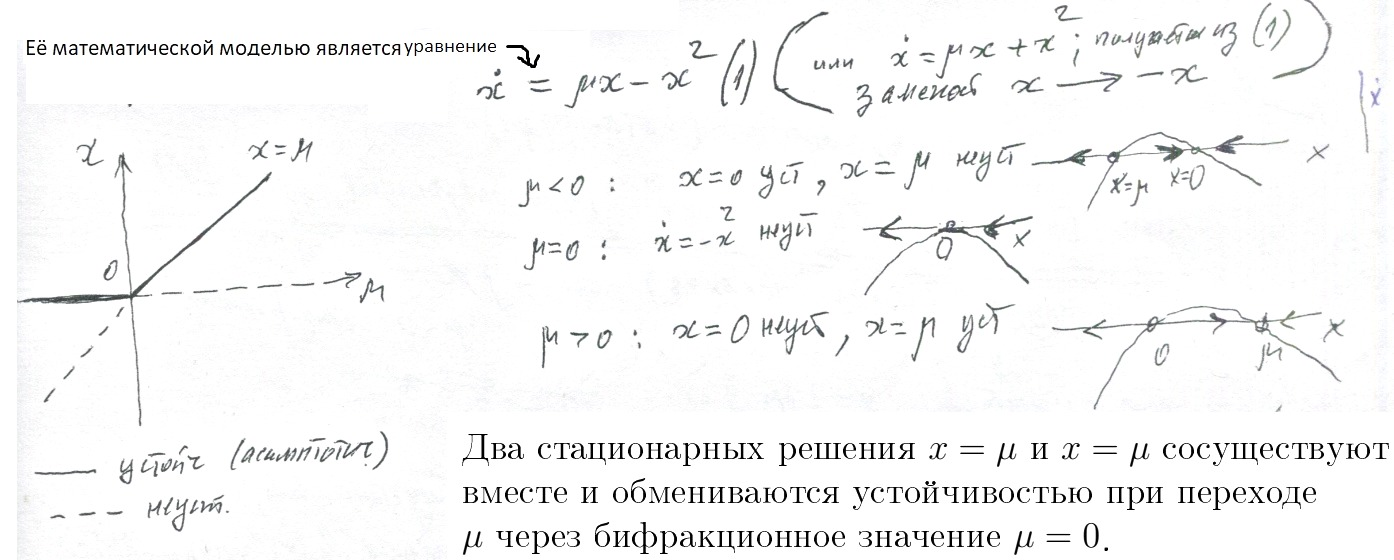
\includegraphics[scale=0.65]{11}

Чтобы получить системы с большей размерностью, надо добавить ещё уравнения, которым отвечает матрица, собственные значения которой отрицательны.


%\[\left\{
%\begin{aligned}
%&\dot{x} ={\mu}x-x^2\\
%&\dot{y} =-y
%\end{aligned}
%\right.
%\]
\begin{wrapfigure}{r}{16cm}
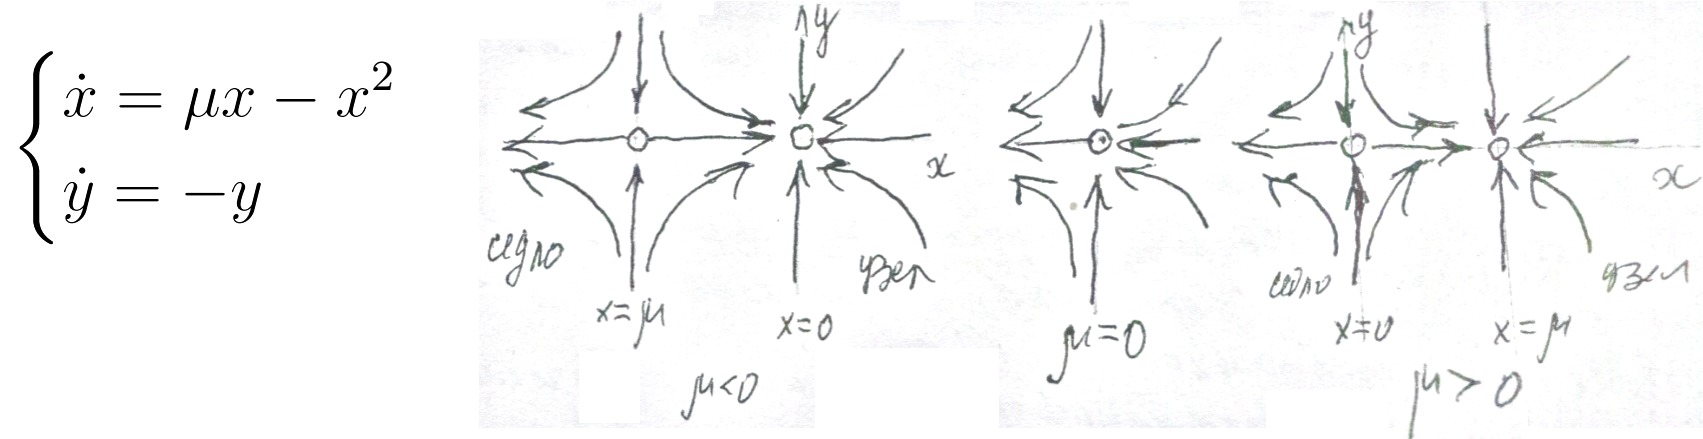
\includegraphics[scale=0.38]{22}
\end{wrapfigure}

|

Например,


пусть

|

|

|

|


|

При переходе через $\mu=0$ седло переходит в устойчивый узел, а устойчивый узел-- в седло.
\section{{\large Бифуркация <<седло- узел>>, или двукратное равновесие}}
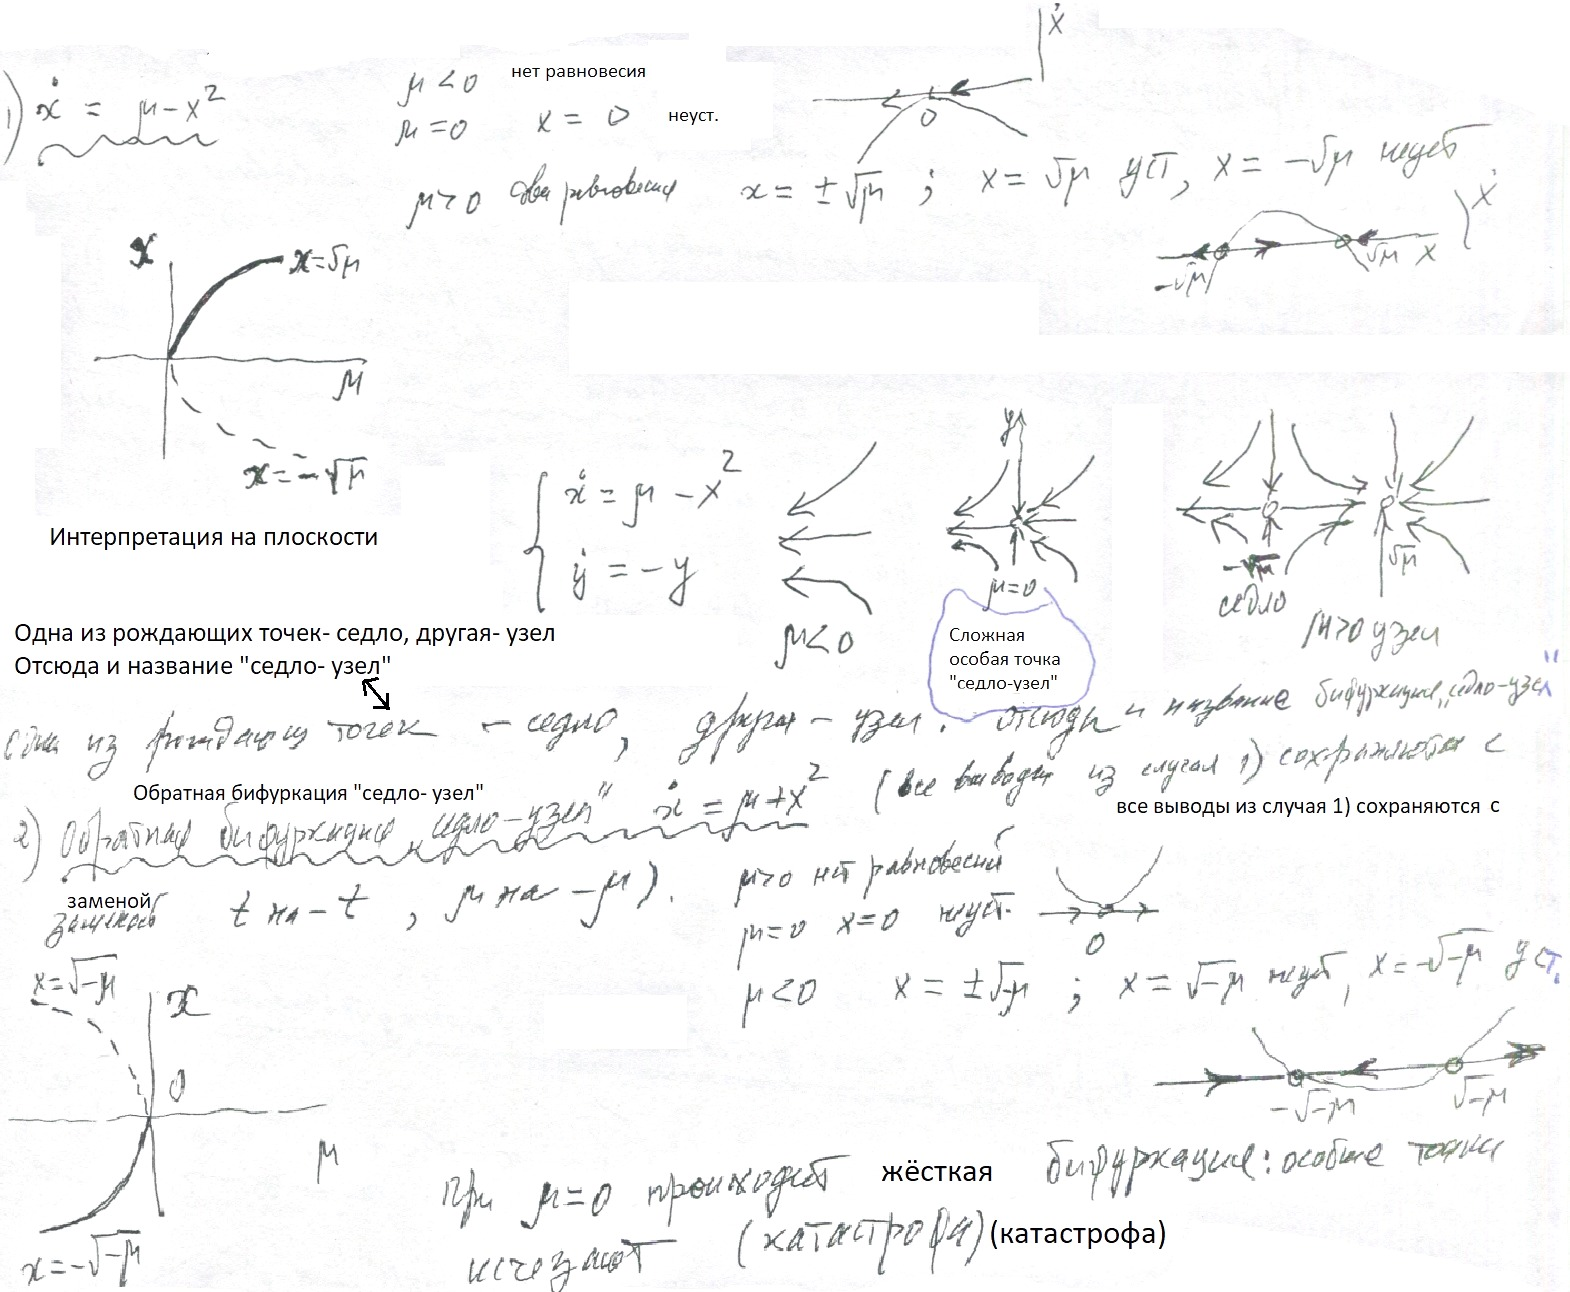
\includegraphics[scale=0.58]{33}
\section{{\large Бифуркация типа<<Вилка>> (или бифуркация <<удвоения>>)}}
1) Прямая бифуркация (надкритическая) \hspace{1cm} $\dot{x}={\mu}x-x^3$\\

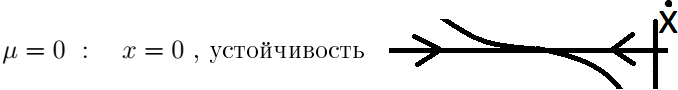
\includegraphics[scale=0.81]{44}


$\mu<0$ -- одно равновесие $x=0$, уст.
\begin{figure}[h!]
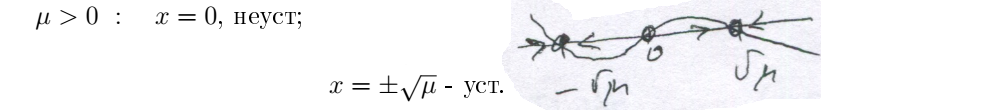
\includegraphics[scale=0.81]{55}
\end{figure}
\begin{wrapfigure}{l}{5cm}
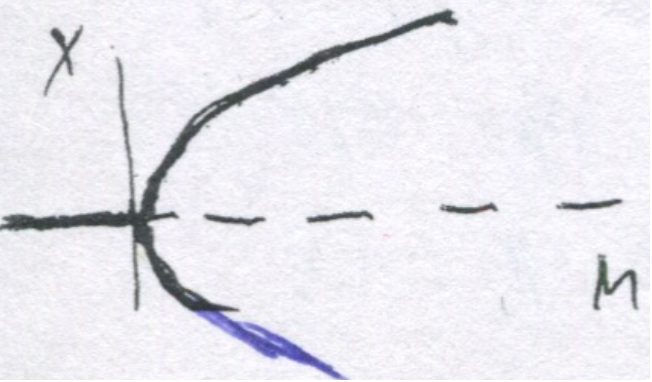
\includegraphics[scale=0.38]{66}
\end{wrapfigure}
Устойчивые точка $x=0$, становясь неустойчивой, пораждает две других устойчивых равновесия. Бифуркационная <<вилка>> здесь она мягкая
\newpage
\begin{figure}[h!]
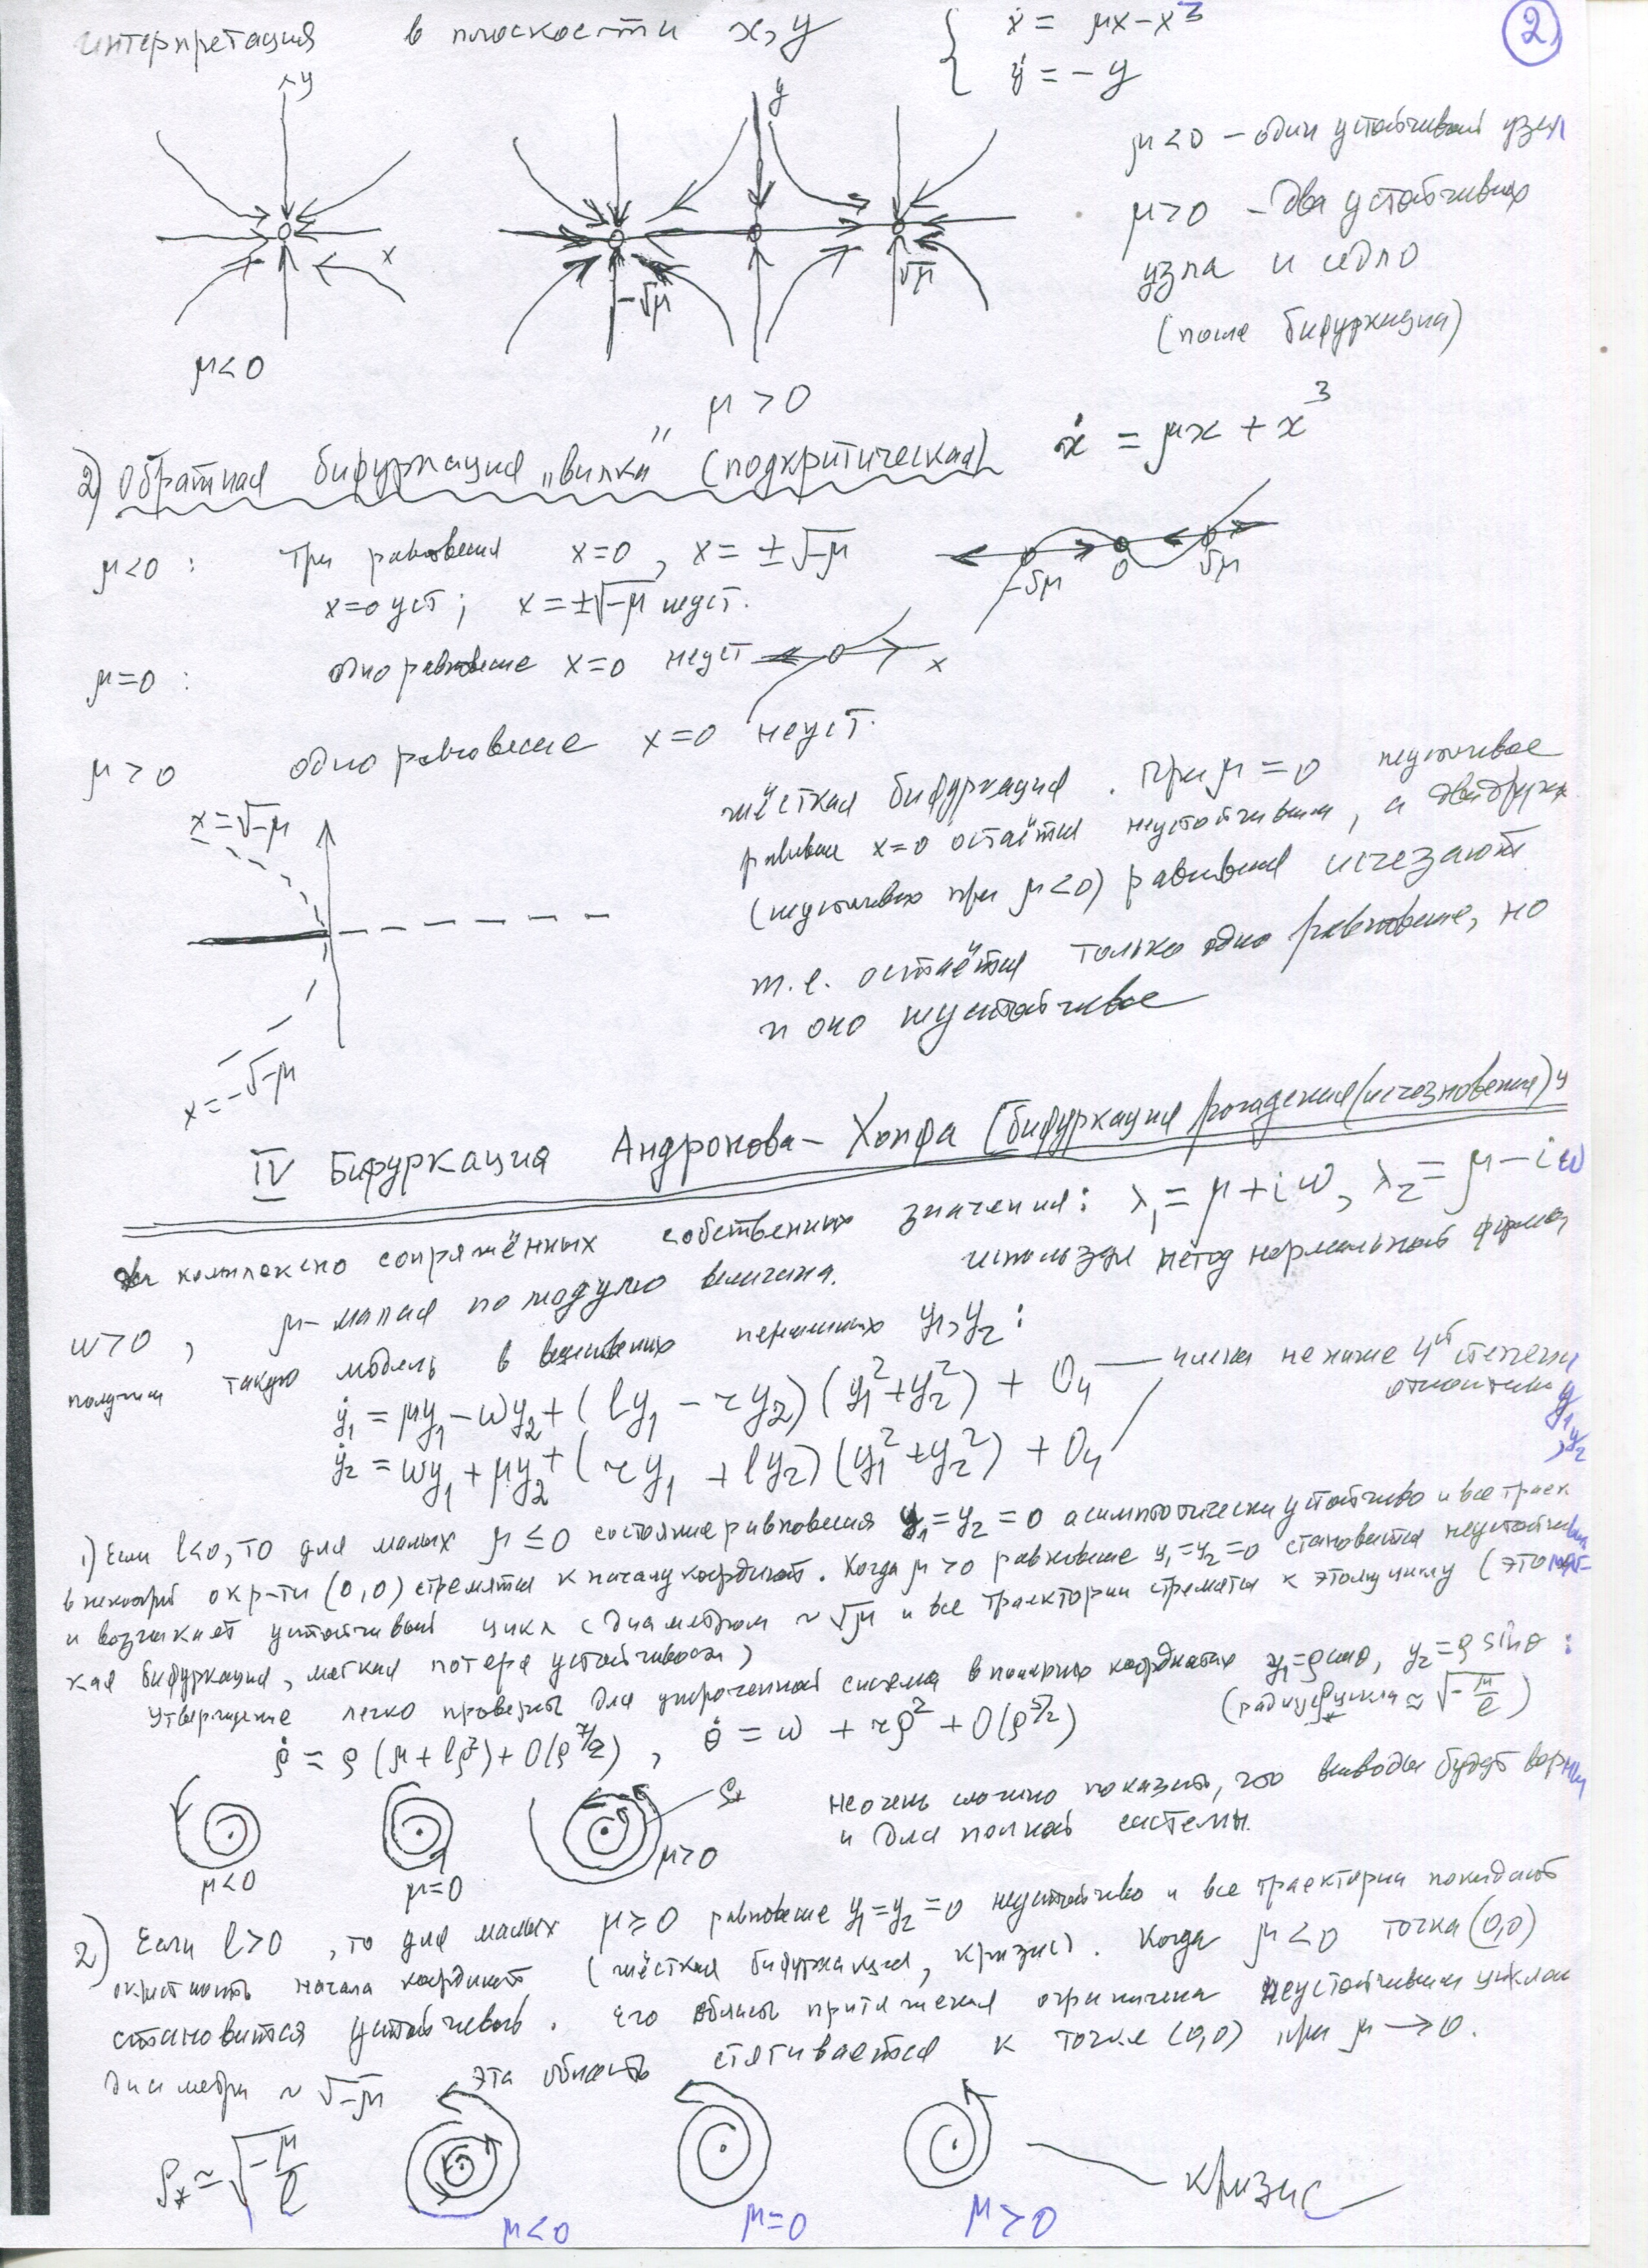
\includegraphics[scale=0.21]{77}
\end{figure}
\end{document}